% Options for packages loaded elsewhere
\PassOptionsToPackage{unicode}{hyperref}
\PassOptionsToPackage{hyphens}{url}
\PassOptionsToPackage{dvipsnames,svgnames,x11names}{xcolor}
%
\documentclass[
  12pt,
]{article}
\usepackage{amsmath,amssymb}
\usepackage{lmodern}
\usepackage{iftex}
\ifPDFTeX
  \usepackage[T1]{fontenc}
  \usepackage[utf8]{inputenc}
  \usepackage{textcomp} % provide euro and other symbols
\else % if luatex or xetex
  \usepackage{unicode-math}
  \defaultfontfeatures{Scale=MatchLowercase}
  \defaultfontfeatures[\rmfamily]{Ligatures=TeX,Scale=1}
\fi
% Use upquote if available, for straight quotes in verbatim environments
\IfFileExists{upquote.sty}{\usepackage{upquote}}{}
\IfFileExists{microtype.sty}{% use microtype if available
  \usepackage[]{microtype}
  \UseMicrotypeSet[protrusion]{basicmath} % disable protrusion for tt fonts
}{}
\makeatletter
\@ifundefined{KOMAClassName}{% if non-KOMA class
  \IfFileExists{parskip.sty}{%
    \usepackage{parskip}
  }{% else
    \setlength{\parindent}{0pt}
    \setlength{\parskip}{6pt plus 2pt minus 1pt}}
}{% if KOMA class
  \KOMAoptions{parskip=half}}
\makeatother
\usepackage{xcolor}
\usepackage[margin=1in]{geometry}
\usepackage{longtable,booktabs,array}
\usepackage{calc} % for calculating minipage widths
% Correct order of tables after \paragraph or \subparagraph
\usepackage{etoolbox}
\makeatletter
\patchcmd\longtable{\par}{\if@noskipsec\mbox{}\fi\par}{}{}
\makeatother
% Allow footnotes in longtable head/foot
\IfFileExists{footnotehyper.sty}{\usepackage{footnotehyper}}{\usepackage{footnote}}
\makesavenoteenv{longtable}
\usepackage{graphicx}
\makeatletter
\def\maxwidth{\ifdim\Gin@nat@width>\linewidth\linewidth\else\Gin@nat@width\fi}
\def\maxheight{\ifdim\Gin@nat@height>\textheight\textheight\else\Gin@nat@height\fi}
\makeatother
% Scale images if necessary, so that they will not overflow the page
% margins by default, and it is still possible to overwrite the defaults
% using explicit options in \includegraphics[width, height, ...]{}
\setkeys{Gin}{width=\maxwidth,height=\maxheight,keepaspectratio}
% Set default figure placement to htbp
\makeatletter
\def\fps@figure{htbp}
\makeatother
\setlength{\emergencystretch}{3em} % prevent overfull lines
\providecommand{\tightlist}{%
  \setlength{\itemsep}{0pt}\setlength{\parskip}{0pt}}
\setcounter{secnumdepth}{-\maxdimen} % remove section numbering
\usepackage{longtable}
\usepackage{graphics}
\usepackage{xparse}
\usepackage{moresize}
\usepackage{setspace}
\usepackage{tcolorbox}
\usepackage{wrapfig}
\usepackage{helvet}
\usepackage{sectsty}
\usepackage{fancyhdr}
\usepackage{xpatch}
\usepackage{booktabs}
\onehalfspacing
\pagestyle{fancy}
\definecolor{gssmidblue}{RGB}{32, 115, 188}
\definecolor{dfeheadingblue}{RGB}{16, 79, 117}
\renewcommand{\familydefault}{\sfdefault}
\allsectionsfont{\color{dfeheadingblue}}
\sectionfont{\color{dfeheadingblue}\fontsize{16}{18}\selectfont}
\fancyhead[C]{}
\fancyhead[RL]{}
\fancyfoot[LR]{}
\fancyfoot[C]{\sffamily \thepage}
\renewcommand{\headrulewidth}{0pt}
\renewcommand{\footrulewidth}{0pt}
\futurelet\TMPfootrule\def\footrule{{\color{gssmidblue}\TMPfootrule}}
\usepackage{floatrow}
\floatsetup[figure]{capposition=top}
\usepackage[tableposition=top]{caption}
\usepackage[titles]{tocloft}
\renewcommand{\cftdot}{}
\AtBeginDocument{\let\maketitle\relax}
\usepackage{cellspace}
\usepackage{etoolbox}
\colorlet{headercolour}{DarkSeaGreen}
\ifLuaTeX
  \usepackage{selnolig}  % disable illegal ligatures
\fi
\IfFileExists{bookmark.sty}{\usepackage{bookmark}}{\usepackage{hyperref}}
\IfFileExists{xurl.sty}{\usepackage{xurl}}{} % add URL line breaks if available
\urlstyle{same} % disable monospaced font for URLs
\hypersetup{
  pdftitle={workshop\_R},
  pdfauthor={Department for Education},
  colorlinks=true,
  linkcolor={Maroon},
  filecolor={Maroon},
  citecolor={Blue},
  urlcolor={blue},
  pdfcreator={LaTeX via pandoc}}

\title{workshop\_R}
\author{Department for Education}
\date{}

\begin{document}
\maketitle

\resizebox{48mm}{!}{
\includegraphics{images/Department_for_Education.png}}

\vspace*{0.24\textheight}

\raggedright\HUGE{\color{dfeheadingblue}\textbf{DfE Statistics Development Team Workshops}} 

\huge{\color{dfeheadingblue}\textbf{Coding RAP using R}}
\vspace*{2\baselineskip} 

\normalsize 
 \newpage 


{
\hypersetup{linkcolor=}
\setcounter{tocdepth}{2}
\tableofcontents
}
\newpage

\hypertarget{introduction}{%
\section{Introduction}\label{introduction}}

We've prepared this walkthrough guide for statistics publication teams
as an introduction to the ways in which coding in R can be used for
Reproducible Analystical Pipelines (RAPs), creating functions for
typical tasks that teams may come across. The guide is intended to be
step-by-step, building up from the very basics. The plan is to work
through this in groups of 3-ish with access to experienced R users for
support. If it starts too basic for your level, then just go through at
your own/your group's pace as you see fit. By no means can we cover
everything in this walkthrough, so please see it as a prompt to ask
follow-up questions as you're working through on anything related to R,
RAP and coding in general.

\hypertarget{what-is-a-rap}{%
\subsection{What is a RAP?}\label{what-is-a-rap}}

RAP stands for Reproducible Analytical Pipeline. The full words still
hide the true meaning behind buzzwords and jargon though. What it
actually means is using automation to our advantage when analysing data,
and this is as simple as writing code such as an R script that we can
click a button to execute and do the job for us.

Using R (the coding language) really helps us to put the R in RAP
(`reproducible'). Ask yourself, if someone else picked up your work,
could they easily reproduce your exact outputs? And when the time comes
around to update your analysis with new data, how easy is it for you to
reproduce the analysis you need? In an ideal RAP, it would be as simple
as plugging the new data in and clicking `go', with no need to manually
scroll through multiple scripts updating the year in every file name or
the variable name that's changed from using \_ to -.

\hypertarget{pre-workshop-requirements}{%
\section{Pre-workshop requirements}\label{pre-workshop-requirements}}

\hypertarget{technical-requirements}{%
\subsection{Technical requirements}\label{technical-requirements}}

First of all, make sure to bring your laptop. This is going to be
interactive and require you to do some coding.

Preferably before coming along, you'll need to go through the following
list of things you'll need to make sure are set up on your DfE laptop:

\begin{itemize}
\item
  Set up an Azure Dev Ops Basic account (not a Stakeholder account) at
  the DfE Service Portal; Either:
\item
  Install git on your laptop: \url{https://git-scm.com/downloads};
\item
  Install R-Studio on your machine: Download \textbf{R for Windows
  (x64)} and \textbf{RStudio} from the Software Centre on your DfE
  laptop.
\end{itemize}

Or:

\begin{itemize}
\tightlist
\item
  If you're on EDAP and used to using R/R-Studio and/or git on there,
  feel free to just use that.
\end{itemize}

You'll also need to make sure that git is set up in the git/SVN pane of
global options in R-Studio (found in the Tools drop down menu). Make
sure the path to your git executable is entered in the git path box and
git should automatically be integrated with R-Studio.

\begin{figure}
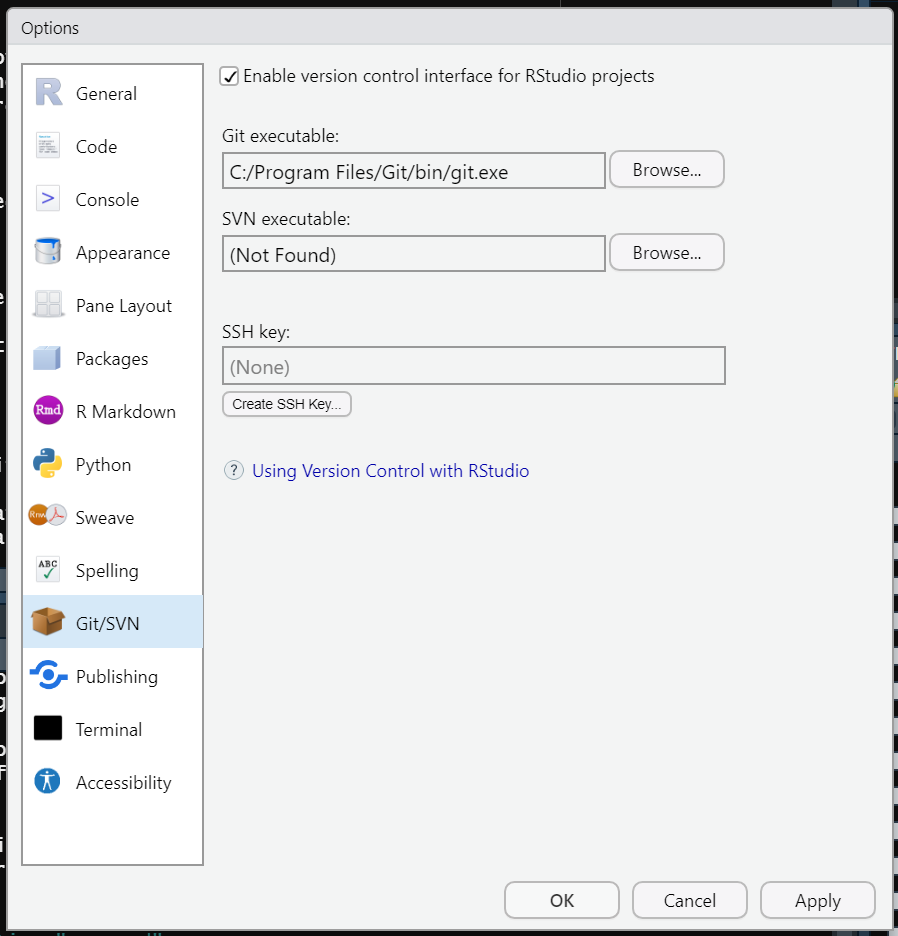
\includegraphics[width=0.64\linewidth]{images/gitdemo/gitdemo-gitRstudio-settings} \caption{Enter the path to your git executable in the git path option box}\label{fig:unnamed-chunk-1}
\end{figure}

Once you open a repository, you'll get an extra panel, named `git', in
the top right pane of R-Studio and you'll also be able to use git in the
`Terminal' tab at the bottom left (in the same place as the R console).

\begin{figure}
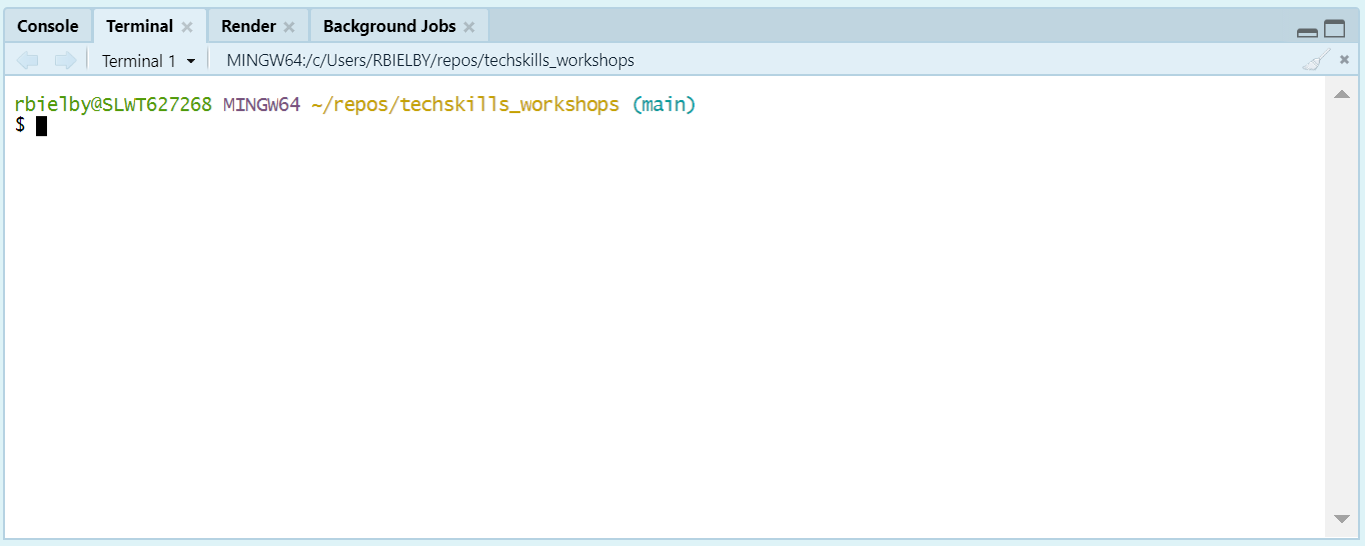
\includegraphics[width=0.56\linewidth]{images/gitdemo/gitdemo-gitRstudio-NewTerminal} \caption{The `git BASH` terminal in R-Studio}\label{fig:unnamed-chunk-2}
\end{figure}

A useful thing here if you want to use git commands in the terminal is
to switch the terminal from the default Windows Command Prompt to
\texttt{git\ BASH}. You can do this in the Terminal tab of R-Studio's
global options - just select \texttt{git\ BASH} from the `New terminal
opens with' pull down menu. Click apply and then select the Terminal tab
(next to the Console tab), click `Terminal 1' and then select `New
terminal' from the drop down menu. You should see something similar to
the terminal screenshot.

\hypertarget{working-in-teams}{%
\subsection{Working in teams}\label{working-in-teams}}

To get the most out of git and Dev Ops, you're going to need to work in
teams. We're aiming for groups of 3. Some of the tasks we'll work
through will require just one of your team to perform, whilst others
will require all of your team to perform them. If it's not clear then
ask and most importantly, communicate with each other about what you're
doing.

To help illustrate the challenges and benefits of git and Dev Ops and
how to work collectively within the same space, all the groups will be
working within the same repository. Each group will have their own
working branch (already created) with the naming format
\texttt{workshop\_group\_N}:

\begin{itemize}
\tightlist
\item
  \texttt{workshop\_group\_1}
\item
  \texttt{workshop\_group\_2}
\item
  \ldots{}
\end{itemize}

We'll need to prefix branches and tasks within the repository with
\texttt{grN\_} and group N respectively (again switching the \texttt{N}
for your group number).

By the end, you should get a good idea of how to utilize R for RAP
processes, as well as how to collaborate using git!

\newpage

\hypertarget{getting-started}{%
\section{Getting started \ldots{}}\label{getting-started}}

Now we will begin the tasks and group work. First, everyone open the R
project that

\hypertarget{summary}{%
\subsection{Summary}\label{summary}}

We've looked through a lot of the basics in this section, covering
adding/staging, committing, pushing/pulling between remote and local
repos, merging and pull requests. These are all the main concepts you
need to use git.

We've also tried to cover doing all this through a mixture of RStudio,
git BASH and GitHub (and as we've said Azure Dev Ops offers similar
functionality to GitHub). Most common processes can be done multiple
ways and there's not necessarily a single right method to follow, just
whichever makes most sense in your situation.

Just a quick final note on why it's useful to be familiar with git
\texttt{BASH}. Whilst most of the basic git functionality can be
accessed via the RStudio panel or GitHub/Dev Ops, there are some things
that are best achieved through BASH. In particular, if you have a file
in your repo that you need to remove entirely, this pretty much requires
someone to use commands via git BASH.

\begin{longtable}[]{@{}
  >{\raggedright\arraybackslash}p{(\columnwidth - 4\tabcolsep) * \real{0.2113}}
  >{\raggedright\arraybackslash}p{(\columnwidth - 4\tabcolsep) * \real{0.4225}}
  >{\centering\arraybackslash}p{(\columnwidth - 4\tabcolsep) * \real{0.3662}}@{}}
\toprule()
\begin{minipage}[b]{\linewidth}\raggedright
Process
\end{minipage} & \begin{minipage}[b]{\linewidth}\raggedright
git BASH
\end{minipage} & \begin{minipage}[b]{\linewidth}\centering
RStudio git panel
\end{minipage} \\
\midrule()
\endhead
Create branch & \texttt{git\ checkout\ -b\ branch\_name} &
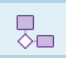
\includegraphics{"images/gitdemo/gitdemo-RStudio-gitToolbarCreateBranch.png"} \\
Switch branch & \texttt{git\ checkout\ branch\_name} &
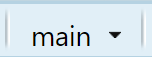
\includegraphics{"images/gitdemo/gitdemo-RStudio-gitToolbarSwitchBranch.png"} \\
Merge branch & \texttt{git\ merge\ branch\_name} & N/A - use GitHub/Dev
Ops \\
\bottomrule()
\end{longtable}

\newpage

\hypertarget{troubleshooting}{%
\section{Troubleshooting}\label{troubleshooting}}

\hypertarget{renv}{%
\subsection{renv}\label{renv}}

If \texttt{renv::restore()} causes issues, then one of your team should
try \texttt{renv::init()} and select option 2 to restart renv. Then do a
add/commit/push cycle and get the other team members to do a pull and
then try running \texttt{renv::restore()} again on their local clones of
the repo.

\hypertarget{datafiles-commit-hooks.gitignore}{%
\subsection{\texorpdfstring{Datafiles
commit-hooks/\texttt{.gitignore}}{Datafiles commit-hooks/.gitignore}}\label{datafiles-commit-hooks.gitignore}}

To help teams keep on top of avoiding any accidental publishing of
unpublished data, we've added in some code around commits that checks
through any data files in the repo and checks them against a logfile and
the .gitignore file. Any files listed in .gitignore will not be included
in commits and therefore won't be sent to the remote repo as part of any
push.

\hypertarget{merge-conflicts}{%
\subsection{merge conflicts}\label{merge-conflicts}}

Merge commits happen when two branches have conflicting changes that
have been made concurrently. \texttt{git} can usually figure out how to
prioritise changes based on the commit history, but if changes have
happened at the same time to the same bit of code across different
branches, then it will need to get your input on how to prioritise the
changes.

The easiest way to go through how to deal with merge conflicts is by
discussing with an example, so ask us in the workshop if and when you
hit a merge conflict.

Briefly though, when there's a merge conflict, git will add some text to
the file containing the conflict along the following lines:

\begin{verbatim}
<<<<<<<<<<< branch_1
code 
on 
branch 
1
===========
conflicting code on branch 2
>>>>>>>>>>> branch_2
\end{verbatim}

Effectively as the user, you need to decide which bit of code is the
right bit to keep and then delete anything you don't want to keep as
well as the tag-lines that git has added in. So for example, you should
be left with something along the lines of:

\begin{verbatim}
code 
on 
branch 
1
\end{verbatim}

Once you've cleared up all merge conflicts in the branch that you're
working on, then perform another add/commit cycle and thay should clear
out the conflict from the branch that you're working on and you'll be
able to continue with the intended merge/PR.

\newpage

\resizebox{48mm}{!}{
\includegraphics{images/Department_for_Education.png}}
\vspace*{\fill}
\color{black}

© Crown copyright 2022

This publication (not including logos) is licensed under the terms of
the Open Government Licence v3.0 except where otherwise stated. Where we
have identified any third party copyright information you will need to
obtain permission from the copyright holders concerned.

To view this licence:

\begin{tabular}{p{0.02\linewidth} p{0.1\linewidth} p{0.88\linewidth}}
& visit & www.nationalarchives.gov.uk/doc/open-government-licence/version/3 \\
& email & psi@nationalarchives.gsi.gov.uk \\
& write to & Information Policy Team, The National Archives, Kew, London, TW9 4DU \\
\end{tabular}

About this publication:

\begin{tabular}{p{0.02\linewidth} p{0.1\linewidth} p{0.88\linewidth}}
& enquiries & www.education.gov.uk/contactus \\
& download & www.gov.uk/government/publications \\
\end{tabular}

\begin{tabular}[t]{p{0.06\linewidth} p{0.24\linewidth} p{0.04\linewidth} p{0.06\linewidth} p{0.36\linewidth}}
\raisebox{-.5\height}{
\includegraphics{images/logoTwitter.png}} &
Follow us on Twitter: @educationgovuk &
&
\raisebox{-.5\height}{
\includegraphics{images/logoFacebook.png}} &
Like us on Facebook: \qquad facebook.com/educationgovuk\\
\end{tabular}

\end{document}
